\documentclass[a4paper]{article}
\usepackage{hyperref}
\usepackage{listings}
\usepackage{graphicx}
\usepackage{comment}


\setlength\parindent{0pt}


\usepackage{color}
\usepackage{subcaption}


\graphicspath{{images/}} %Setting the graphicspath

\def\code#1{\texttt{#1}}
\newcommand{\fig}{Fig.~}	% figure ref
\newcommand{\eqn}{Eq.~}	% equation ref
\newcommand{\tab}{Tab.~}	% table ref
\newcommand\red[1]{{\textcolor{red}{#1}}}


\title{Algoritmi di Brain Computer Interface per il controllo di sistemi domotici}
\author{Dario Sanalitro \\  \url{dariosanalitro@hotmail.it}}
\date{31/01/2023}




\begin{document}
	\maketitle

\newcommand{\agrave}{\'a~}
\newcommand{\aacuto}{\`a~}
\newcommand{\egrave}{\`e~}
\newcommand{\uacuto}{\`u~}
\newcommand{\iacuto}{\`i~}
\newcommand{\oacuto}{\`o~}

\section{Introduzione e Scelte progettuali}

Nel contesto del progetto "Algoritmi di Brain Computer Interface per il controllo di sistemi domotici" che rientra all'interno del progetto di ricerca "Ricerca e Innovazione” – Progetto “\textit{4 FRAILTY –Sensoristica intelligente, infrastrutture e modelli gestionali per la sicurezza di soggetti fragili}" \egrave stato realizzato un sistema che permette di acquisire segnali che rilevano l'attivit\aacuto elettrica celebrale tramite interpretazione dell'elettroencefalogramma acquisito per via di elettrodi posizionati a contatto con lo scalpo. Successivamente una fase di processamento dei signali ed una classificazione ne permettono l'utilizzo per un controllo attivo di un sistema domotico caratterizzato da un interruttore e da un gestore di luminosit\aacuto.

Tale sistema trova applicazione in diversi scenari quali l'utilizzo in ambienti e sistemi di controllo intelligenti, movimento di bracci robotici, controllo di moto e pianificazione di veicoli autonomi o semi-autonomi (come sedie a rotelle)  e fornisce un potenziale ed allo stesso tempo concreto aiuto a soggetti affetti da disordini neurologici e congnitivi come sclerosi, ictus, infortuni alla colonna vertebrale, che interrompono le comunicazioni dell'apparato neuromuscolare~\cite{2004-Pfu}.

Per quanto concerne il rilevamento dei segnali provenienti dall'attivit\aacuto celebrale, diverse metodologie sono presenti nello stato dell'arte che possono essere impiegate~\cite{2006-Hoc}. Tra queste le principali sono elettroencefalografia, elettrocortigrafia, magneto-encefalografia, tomografia ad emissione di positrone, spettroscopia vicina agli infrarossi, risonanza magnetica funzionale.

Nell'ambito di questo progetto, la prima, ovvero l'elettroencefalografia, \egrave stata individuata come la pi\uacuto indicata in quanto rappresenta una metodologia non invasiva, portabile, di semplice applicazione e dai costi conenuti. In dettaglio, tale metodologia prevede che il soggetto indossi in testa una rete di sensori con un sistema di pre-amplificazione che a contatto con lo scalpo umano acquisisce l'attivit\aacuto elettrica celebrale. 

Si presenta quindi il problema dell'interpretazione di questi dati che permetta di stabilire una correlazione tra il segnale acquisito e l'intezione espressa mentalmente dal soggetto durante l'acquisizione.
La difficolt\aacuto principale dei sistemi BCI sta nello stabilire metodologie valide per l'estrazione di informazioni relative ad un evento provenienti da segnali elettroencefalografici. La maggior parte dei sistemi BCI basati su elettroencefalografia fa riferimento a diverse tipologie di segnali per tradurre l'intento del soggetto in comandi. Tra queste "\textit{Motor Imagery}"~\cite{2009-Tho} (MI), un segnale che rappresenta lo stato durante il quale la rappresentazione di una specifica attivit\aacuto motoria \egrave internamente riattivata in memoria, la componente P300~\cite{2008-Len} che rappresenta una specifica componente dei segnali elettrici acquisiti e che si manifesta ogni qual volta vi \egrave una risposta ad uno stimolo definibile "importante", "\textit{Visually Evoked Potentials}" (VEP) e pi\uacuto in dettaglio "\textit{Steady-State Visually Evoked Potentials}"~\cite{2013-Xia} che rappresentano segnali acquisiti a seguito di un'esposizione da parte del soggetto a stimoli oscillanti visuali.

Nel contesto specifico del progetto in esame, l'attivit\aacuto mentale utilizzata \egrave stata il MI in quanto tali segnali, essendo basati su analisi in frequenza, presentano la caratteristica di avere tempi di risposta celeri che risultano essere ideali nel caso si vogliano espletare delle azioni ben precise, come ad esempio comandare un interruttore o un dosatore di livello dell'intensit\aacuto della luce.
Sebbene tale approccio richiede una la lunga procedura nella classificazione  dei segnali, la scelta progettuale effettuata \egrave stata quella di spostare la complessit\aacuto nella fase di processamento dei dati e progettazione dell'interfaccia con l'utente.

Successivamente alla fase di acquisizione dei segnali, in generale, seguono una fase di pre-processamento e post-processamento ed una fase di classificazione che permettano l'identificazione di parametri robusti da correlarsi con l'attivit\aacuto mentale del soggetto in esame.

Nella fase di pre e post-processamento, si manipolano i segnali acquisiti per poter principalmente separare la parte significativa dei segnali dal rumore di fondo e rimuovere gli artefatti provenienti dalle attivit\aacuto oculari e muscolari. Nell'ambito del progetto in esame, sono stati utilizzati un filtro passa banda nel primo caso ed una metodologia regressiva chiamata "Independent Component Analysis" per i secondi~\cite{2016-Dif}.

Nella fase di classificazione si utilizza classificatori intelligenti o adattivi in grado di processare e classificare i vari segnali. Lo stato dell'arte tra le varie tecniche presenta il cos\iacuto detto modello nascosto di Markov~\cite{2018-Li} e la versione autoregressiva~\cite{2010-Arg}, cos\iacuto come filtri di Kalman o Analisi dei Discriminanti Lineare~\cite{2014-Dua}. Nel caso specifico del progetto, quest'ultima \egrave stata la tecnica utilizzata per estrarre le componenti che rappresentano i segnali grezzi per poi utilizzare un algoritmo di apprendimento automatico per classificare tali componenti e associarle a specifici comportamenti.

\section{Fase Sperimentale}

\subsection{Setup Sperimentale}
Il sistema utilizzato per la validazione sperimentale, di cui una rappresentaione schematica \egrave presentata in~\fig\ref{fig:scheme} consiste in un elmetto EMOTIV EPOC in grado di acquisire l'elettroencefalogramma tramite 14 canali dislocati all'interno dello stesso per via del software EMOTIV PRO. Tali segnali sono stati poi post-processati e classificati tramite una piattaforma software dedicata alla progettazione, sviluppo e test di signali celebrali, chiamata OpenVibe\footnote{http://openvibe.inria.fr/}. Con il fine ultimo di fornire una piattaforma facilmente utilizzabile da qualsiasi utente, Node-red\footnote{https://nodered.org/}, che rappresenta un tool di sviluppo per la programmazione e la interconnessione di dispositivi, interfaccie software e servizi online ed un protocollo di comunicazione "open-source" altamente adoperato in applicazioni di domotica ("KNX Protocol") sono stati utilizzati per la gestione dei comandi con l'interruttore ed il regolatore di luminosit\aacuto Schneider Electric MTN647395 e MTN649350 come mostrato in~\fig\ref{fig:exp}.

\subsection{Validazione Sperimentale}

In particolare, la validazione sperimentale ha avuto luogo in quattro fasi: un fase di registrazione dei segnali elettroencefalogrifici, una fase di apprendimento della rete neurale per l'interpretazione di tali segnali, una fase cos\iacuto detta di prova che permette di valutare l'accuratezza della classificazione effettuata dalla rete neurale, ed una quarta e finale fase in cui il soggetto pu\oacuto interagire direttamente con i dispositivi a disposizione.
 
Durante la prima fase di registrazione, il soggetto si \egrave allenato su attivit\aacuto specifiche utilizzando un opportuno protocollo. In particolare, il soggetto \egrave stato sottoposto ad una serie continuativa di stimoli visivi, ovvero una freccia a sinistra ed una freccia a destra per un totale di 7 minuti, in maniera che i segnali elettroencefalografici potessero essere acquisiti. Questa fase, in virt\uacuto dell'utilizzo di MI \egrave in generale particolarmente importante ai fini della riuscita dell'esperimento. Nello specifico, tale fase \egrave consistita in uno stimolo visivo di una durata di circa 7 secondi sullo schermo all'interno della quale \egrave richiesto al soggetto di trovare una strategia mentale che permetta di differenziare l'attivit\aacuto corticale registrata durante la presentazione dei due stimoli visivi.

Successivamente alla fase di registrazione, l'algoritmo ha fornito come risultato i pesi della rete neurale necessari a creare i parametri correttivi relativi al soggetto che ha effettuato la fase di registrazione. Tali parametri sono stati salvati ed utilizzati nella fase successiva, ovvero la fase di prova in cui al soggetto, a seguito dell'apparizione a schermo di una freccia a sinistra o a destra, viene richiesto di discernerne il verso. Un riscontro in tempo reale ed un'analisi di accuratezza della procedura sono stati il risultato di questa terza fase. 

In seguito alla validazione dell'accuratezza e alla valutazione della validit\aacuto dei parametri relativi al soggetto che ha eseguito il test, \egrave stato possibile comandare l'interruttore e il regolatore di luminosit\aacuto da parte del soggetto in esame come mostrato in~\fig\ref{fig:exp}. 

\begin{figure}[t]
	
\includegraphics[width=\textwidth]{block-scheme.png}
	\caption{Schema a blocchi dell'architettura hardware e software utilizate nell'ambito del progetto per realizzare un sistema domotico basato su BCI}
	\label{fig:scheme}
\end{figure}

\begin{figure}[t]
	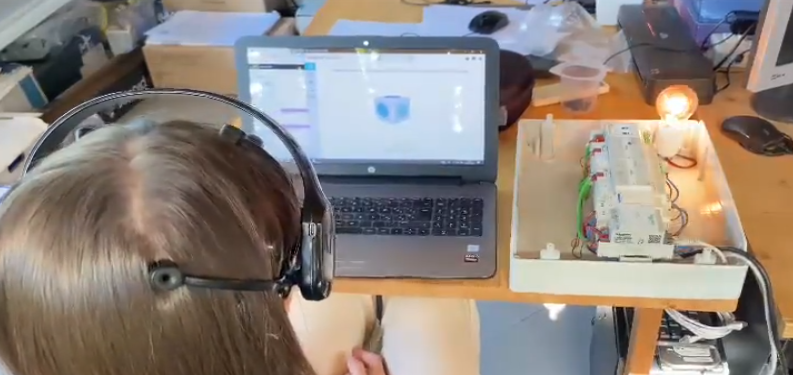
\includegraphics[width=\textwidth]{real-exp.png}
	\caption{Realizzazione esperimento di controllo di un interrutorre on-off e di un regolatore di luminosit\aacuto}
	\label{fig:exp}
\end{figure}



\bibliography{./bibCustom.bib}
\bibliographystyle{IEEEtran}	

\end{document}
